\documentclass[pdftex,12pt,letter]{article}
\usepackage[binary-units=true]{siunitx}
\usepackage[margin=0.75in]{geometry}
\usepackage[utf8]{inputenc}
\usepackage[T1]{fontenc}
\usepackage{graphicx}
\usepackage{amsmath}
\usepackage{xspace}
\usepackage{xcolor}
\usepackage[pdftex,pdfpagelabels,bookmarks,hyperindex,hyperfigures]{hyperref}

\newcommand{\fixme}[1]{\textcolor{red}{\textit{Fixme}: \textbf{#1}}}


\author{Brett Viren}
\date{\today}
\title{Single-Phase protoDUNE TPC \\ Detector Element Connectivity}
\begin{document}

\maketitle

\begin{abstract}
  \noindent The connectivity of detector elements relevant to TPC wire
  data from the single-phase protoDUNE experiment is described.  It is
  expressed as a directed graph of ordered edges.  Edges map to
  connections between detector elements following numbering conventions
  taken from the engineering designs for the hardware involved.  A
  scheme for flattening this graph and producing a global numbering
  convention is proposed.  The software to produce the graph is
  described and a sample of the diagrams it generates are included for
  validation purposes.
\end{abstract}

%\newpage
\tableofcontents
\newpage
\section{Overview}

This document describes a \textit{directed graph} representing the
connections between the detector elements (aka parts) of the
single-phase protoDUNE detector related to TPC wire data.  Nodes in
the graph are limited to representing those particular detector
elements which have importance for analyzing and simulating the
detector data.  An edge represents a logical or physical connection
between two types of parts and carries index attributes which
represent an ordering of the connection among others of the same type.
As such, the nodes of this graph themselves carry no identifiers but
are identified by their location in the graph.

In determining the connectivity between nodes, the edges and their
indices are chosen to follow engineering and design documents and
drawings.  This allows the graph representation to be independent of
any global numbering convention while still correctly representing the
design.  It also allows representing connectivity which deviates from
design as may arise from mistakes during construction or DAQ
configuration.

The edge index attributes assert a very minimal and connection-local
convention.  This does not preclude more prescriptive or global
conventions to be defined as a function of the resulting graph.
Indeed, multiple useful conventions must likely emerge from this graph
depending on the context in which the connection information is
needed.  For example, waveform data will be associated with a tuple of
numbers (APA, WIB, WIB slot, board, chip, channel) while for
reconstruction and simulation it is important to identify a waveform
with a wire segment described by a different tuple (APA, face,
plane, conductor, segment).  The mapping between any pair of these
tuples is not trivial and requires a graph traversal.

That said, it is also useful to develop conventions to provide a flat
sequence of numbers which enumerate parts at some more global scale.
For example, it is expected that numbering the 400, 400 or 480
``spots'' where a conductor terminates on wire boards in one of the
three planes, respectively, in an APA face will be a useful
intermediate flat numbering scheme for producing visualizations of
waveform samples vs time.  While the wrapping of the induction
conductors will lead to some ambiguity this will give much more
understandable views of the data than would plotting waveforms ordered
by board-chip-channel.

The rest of this section defines the detector elements considered in
the connectivity graph as well as orientation labels and coordinate
system conventions used.  Next, each type of connection is described
in some detail.  Then, schemes for generating ``flat'' or global
numbering conventions are presented.  Finally, some description of the
software used to generate, visualize and validate the connection graph
is provided.


\subsection{Detector Elements}
\label{sec:parts}

Figure~\ref{fig:schema} shows a schema graph which illustrates the
node and edge types that are employed in the full connectivity graph.
The full connectivity graph can be understood as an expansion of this
schema graph over the multiplicities indicated in the nodes and
following proper design ordering.

\begin{figure}[h]
  \centering
  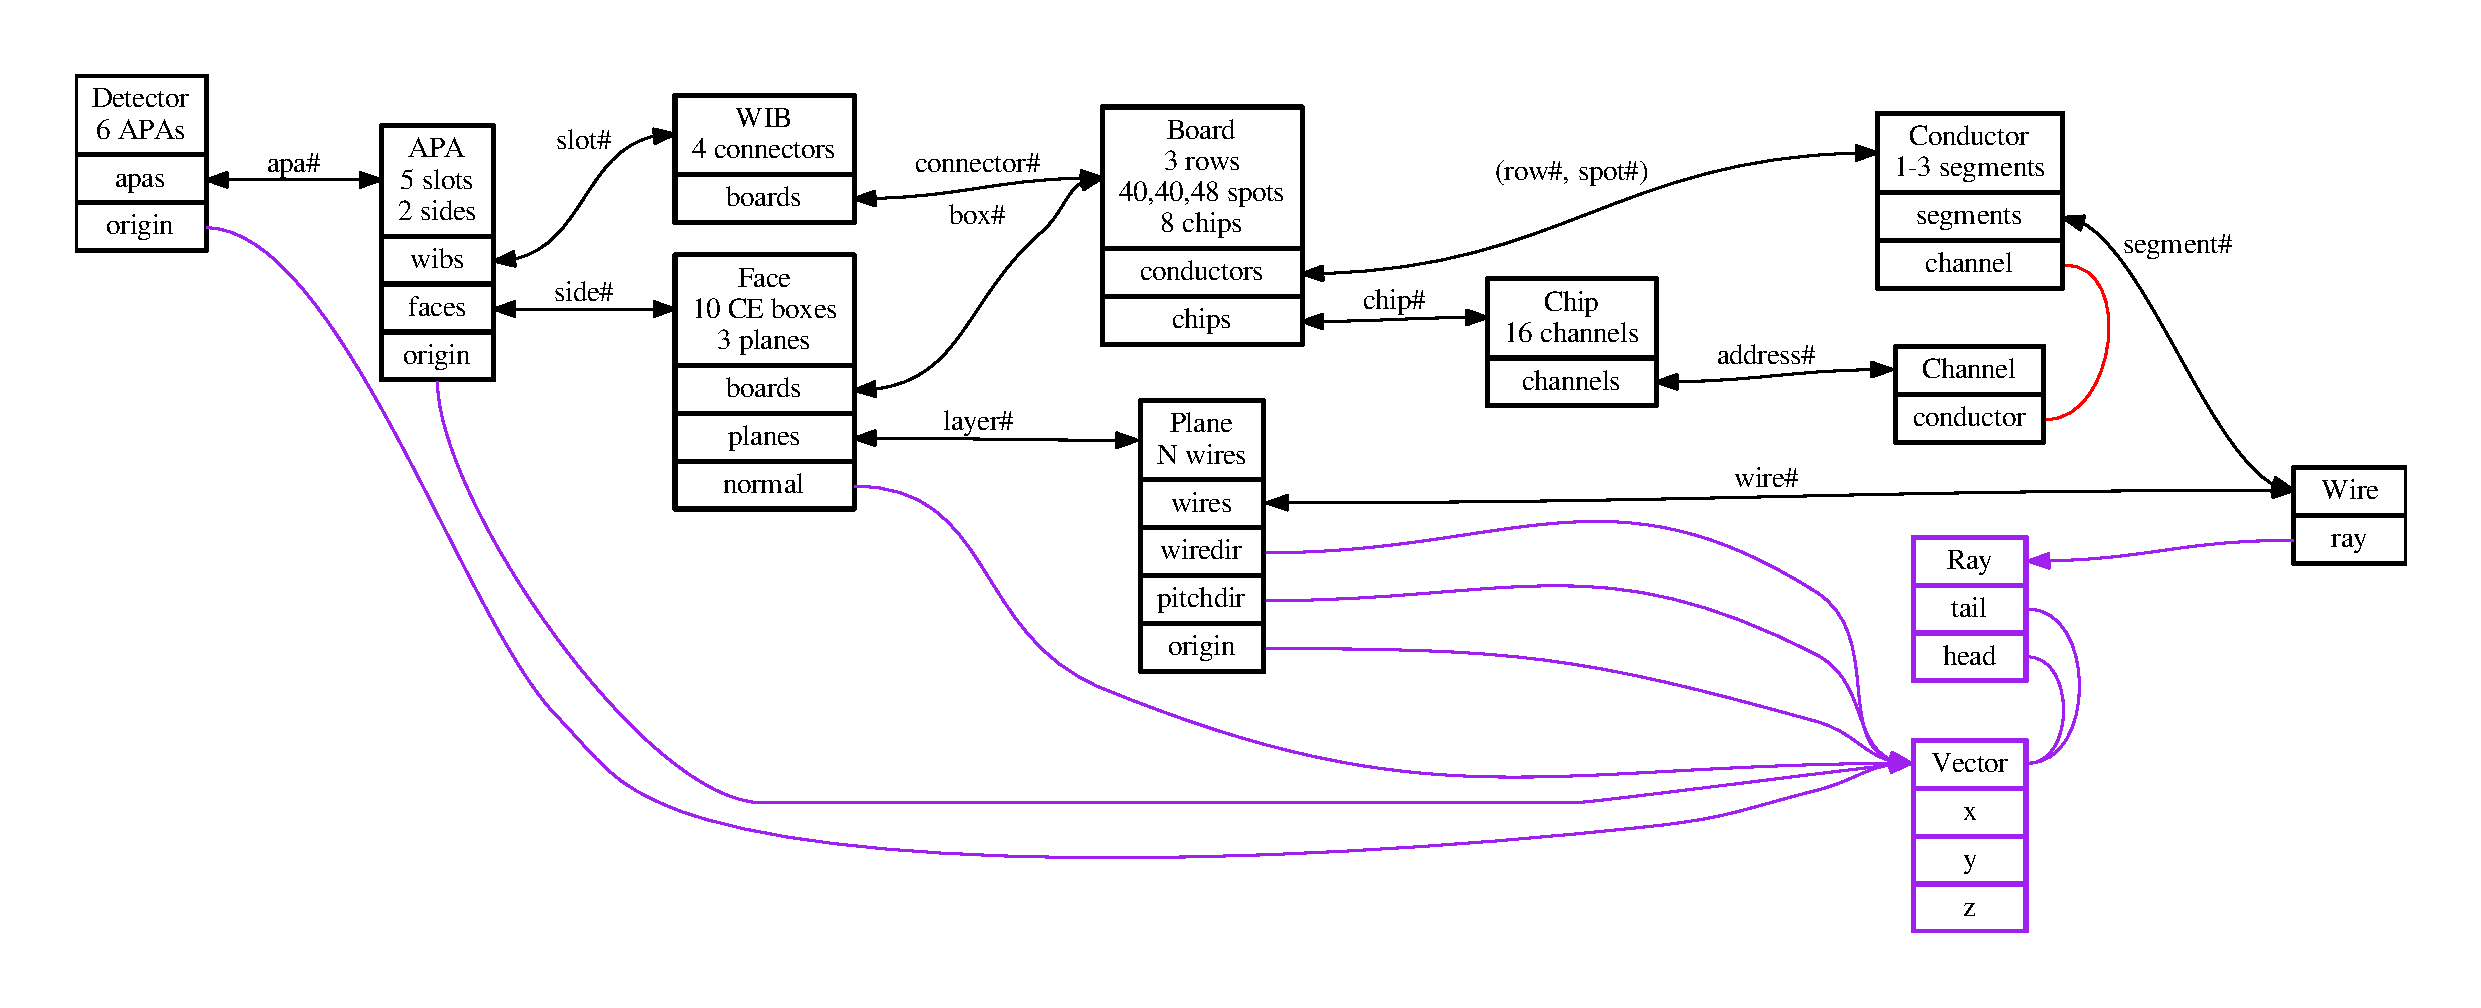
\includegraphics[width=\textwidth]{dots/schema2.pdf}
  \caption[Connectivity schema graph.]{Summary of the schema which the connectivity graph follows.  Black arrows indicate a parent/children relationship.  The relationship has attributes (indices) which allow for ordering and association with physical connectivity.   Purple indicate associated geometry information and red indicate one-to-one relationships. }
  \label{fig:schema}
\end{figure}

The nodes in the schema graph and their multiplicity of association
are described as follows:

\begin{description}

\item[Detector] contains six \textbf{APAs} uniquely identified by
  \texttt{apa\#}.  The location of the detector in global coordinates
  (see below) is given by the \texttt{origin} vector.

\item[APA] is the anode plane assembly, here associated with one crate
  holding five \textbf{WIBs} identified by their \texttt{slot\#} and
  \textbf{faces} identified by \texttt{side\#}.  The location of the
  center of the APA expressed in the detector coordinate system is
  given by the \texttt{origin} vector.

\item[WIB] is a warm interface board with four connections, each to
  one board and, identified by \texttt{connector\#}..

\item[Face] is a logical construct which has ten boards associated by
  \texttt{box\#} and three associated planes with \texttt{layer\#}.
  The direction normal to the face is held in the \texttt{normal}
  vector.

\item[Board] represents a cold electronics front end motherboard
  (FEMB) or equivalently a wire board.  A board has eight chips
  attached and associated through a \texttt{chip\#}.  Conductors are
  attached in one of three rows (\texttt{row\#}), each with 40, 40 or
  48 spots \texttt{spot\#}), respectively.

\item[Plane] is defined by an ordered sequence of coplanar and
  nominally parallel wire segments (associated through
  \texttt{wire\#}).  The direction that the wires run
  (\texttt{wiredir}) and the direction of their pitch
  (\texttt{pitchdir}) are specified as perpendicular vectors in the
  plane.  The location of the active center of the plane with respect
  to the APA center is given in the \texttt{origin} vector.

\item[Chip] a cold electronics chip represents a pair ASICs, one
  front-end amplifier and one cold ADC.  A chip is associated through
  16 channels via the \texttt{channel\#}.

\item[Channel] represents a unique signal input to the chip.  It is
  associated to exactly one conductor.

\item[Conductor] represents a length of sensing wire. It consisting of
  one, two or three wire segments depending on where in and to which
  plane it contributes through the \texttt{segment\#} number.  It is
  associated with exactly one channel.

\item[Wire] represents one segment of a conductor strung across the
  APA frame.  A wire joins the ``data'' hierarchy rooted in a crate of
  WIBs and the ``physical'' hierarchy rooted in the faces of planes.
  As such, a wire can be considered to represent three conceptual
  descriptions.  As part of a conductor, a wire has a segment number
  which counts how many other wires are between it and the attachment
  spot of its conductor.  As part of a plane, a wire has an index into
  an ordered list of wires that make up the plane such that the center
  of the index-zero wire has the smallest possible (most-negative)
  position along the pitch direction of the plane.  Finally,
  geometrically it is defined as a ray in space which points along the
  wire direction of the plane.
\end{description}

\subsection{Orientation}

The installation group has defined an orientation labeling scheme
which is partly adopted here as well.  It defines labels by
considering the detector approximately aligned with the general
direction of the particle beam from CERN.  It is reproduced in
table~\ref{tab:global}.

\begin{table}[htp]
  \label{tab:global}
  \centering
  \begin{tabular}[h]{|c|c|c|}
    \hline
    \multicolumn{3}{|c|}{North, aka ``Beam-Left'' (BL)} \\
    \hline
    Upstream (US) & Midstream (MS) & Downstream (DS) \\
    \hline
    \multicolumn{3}{|c|}{South, aka ``Beam-Right'' (BR)} \\
    \hline
    \multicolumn{3}{c}{$\longrightarrow$ approximate beam direction $\longrightarrow$} \\    
  \end{tabular}
  \caption{Global orientation labels from the installation group.
    Beam travels approximately left to right.  Up-, mid- and
    down-stream may be abbreviated US, MS and DS, respectively.
    Beam-left (BL) and beam-right (BR) are on the North and South
    sides of the detector, respectively.}
\end{table}

\subsection{Coordinate Systems}
\label{sec:coordsys}

A family of Cartesian coordinate systems is adopted in this note to
represent the location of wire segment endpoints.  Their coordinates
are defined and their semantic meanings are summarized as:

\begin{description}
\item[Global] $(x_g, y_g, z_g)$ is associated with some ``lab frame''
  but need not be defined further here.
\item[Detector] $(x_d, y_d, z_d)$ is defined with respect to the
  \textit{global} system and has axes aligned with the detector such
  that $y_d$ points upward, counter to gravity, $z_d$ points
  transverse to the nominal drift direction and approximately in the
  direction of the beam and $x_d$ follows from the right-hand-rule and
  is either parallel or anti-parallel to the nominal (local) electron
  drift direction.  The origin of this coordinate system is left
  unspecified in this document but is what would be provided by the
  \texttt{Detector:origin} as found in 
  Fig.~\ref{fig:schema}.
\item[Chamber] $(x_c, y_c, z_c)$ is defined with respect to the
  \textit{detector} coordinate system.  There is one chamber
  coordinate system for each face-0 TPC drift region of each APA.  For
  each chamber, the $y_c$ direction is parallel to that of the
  \textit{detector} system, the $x_c$ direction is along the normal to
  APA face-0 and $z_c$ follows from right-hand-rule.  The origins of
  both the $y_c$ and $z_c$ axes are chosen to be at the center of the
  active area of the APA face.  The $x_c$ origin lies on the center
  plane that divides the APA into two faces.  
\item[Wire] $(x_w, y_w, z_w)$ is defined with respect to a
  \textit{chamber} coordinate system.  There is one wire coordinate
  system associated with each wire plane in the APA face bounding the
  chamber.  The $x_w$ axis is identified with $x_c$.  The $y_w$ axis
  points along the wire in the direction (positive) current flows
  toward the electronics.  The $z_w$ follows from the right-hand-rule
  and points in the direction of the \textit{wire pitch}.  The origin
  of the wire coordinate system is identified with that of the chamber
  system.  They are related by a rotation but not a
  translation.  Note, for W-planes, the wire and chamber coordinate
  systems are identical.
\end{description}

\noindent These last two categories of coordinate systems are illustrated in Figure~\ref{fig:coords}.

\begin{figure}[htp]
  \centering
  \begin{minipage}[t][10cm][t]{0.59\textwidth}
    \begin{center}
      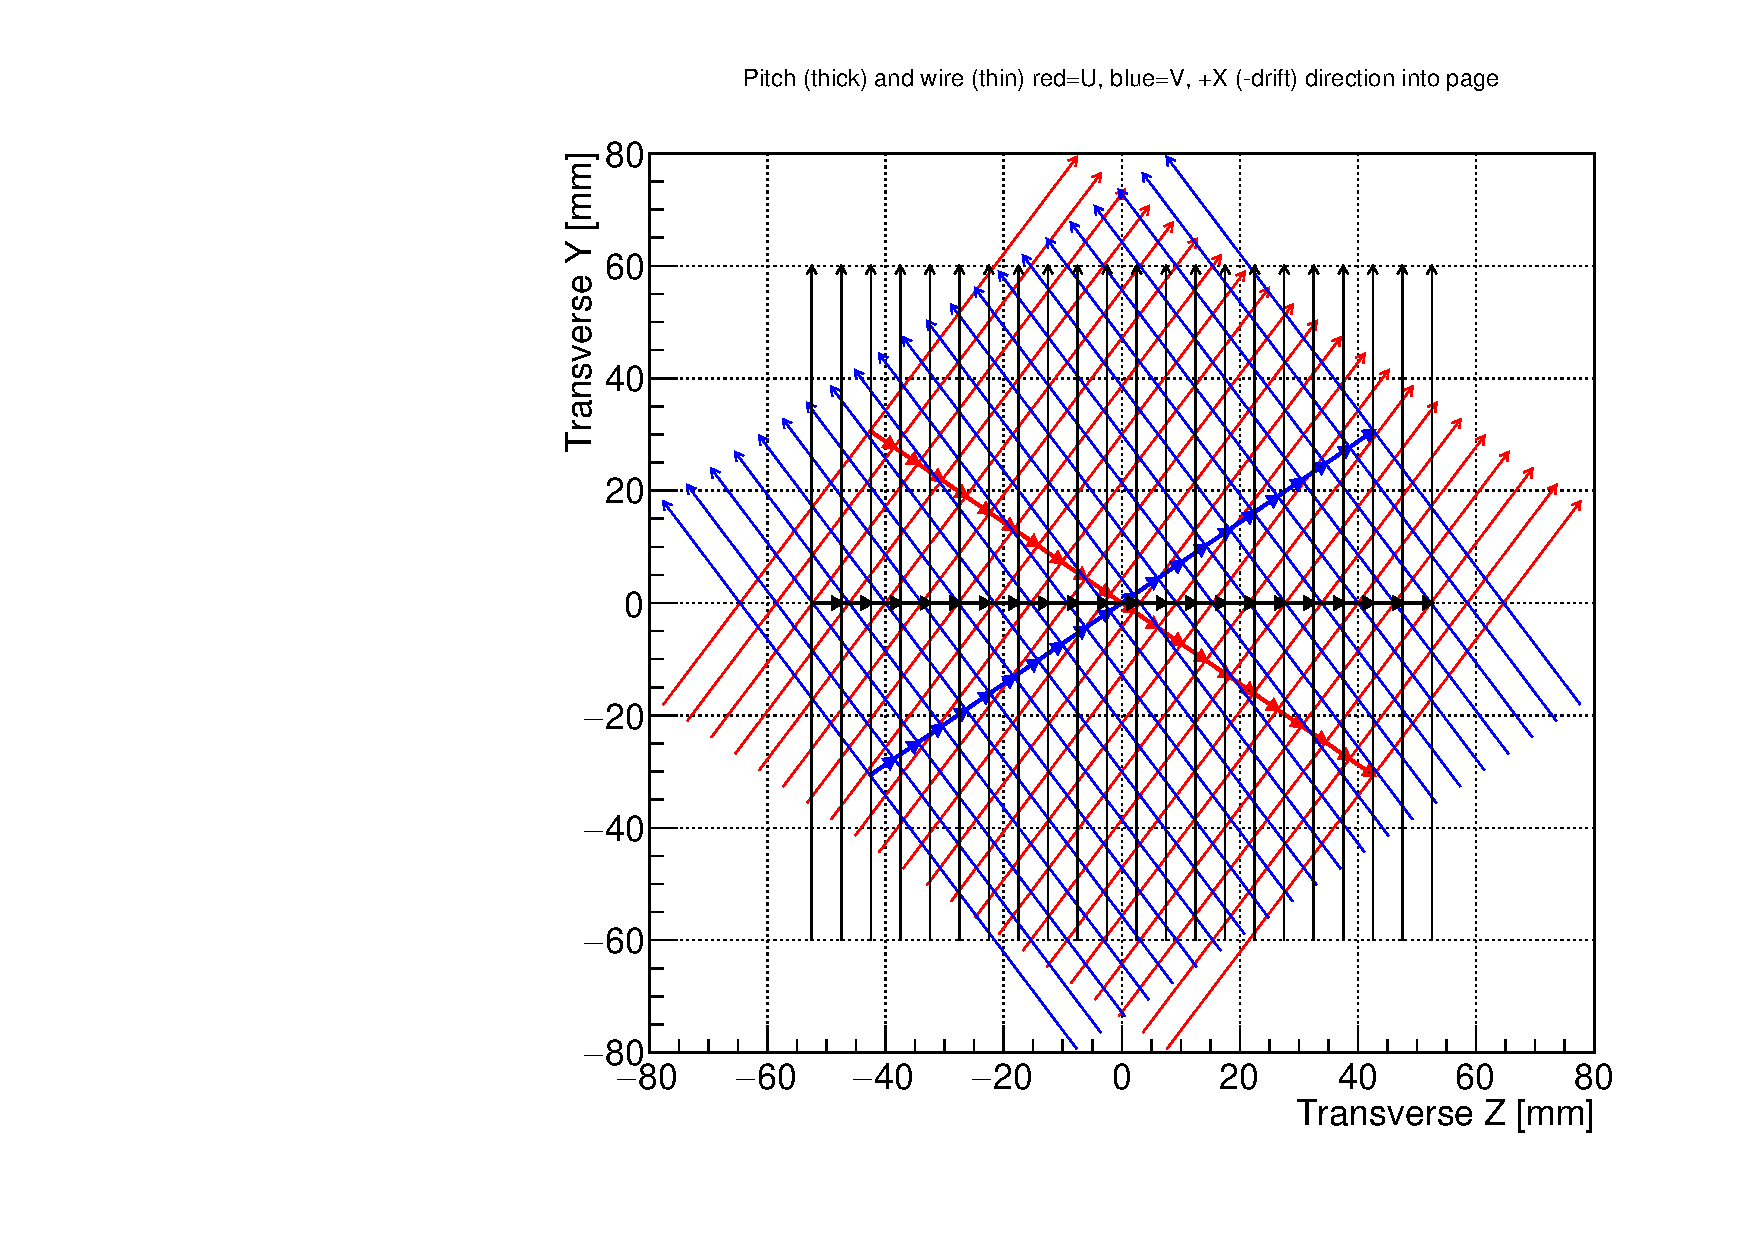
\includegraphics[height=9cm]{test_pimpos_draw.pdf}

      $-z_w \longrightarrow 0 \longrightarrow +z_w$
    \end{center}
  \end{minipage}
  \begin{minipage}[t][10cm][t]{0.39\textwidth}
    \begin{center}
      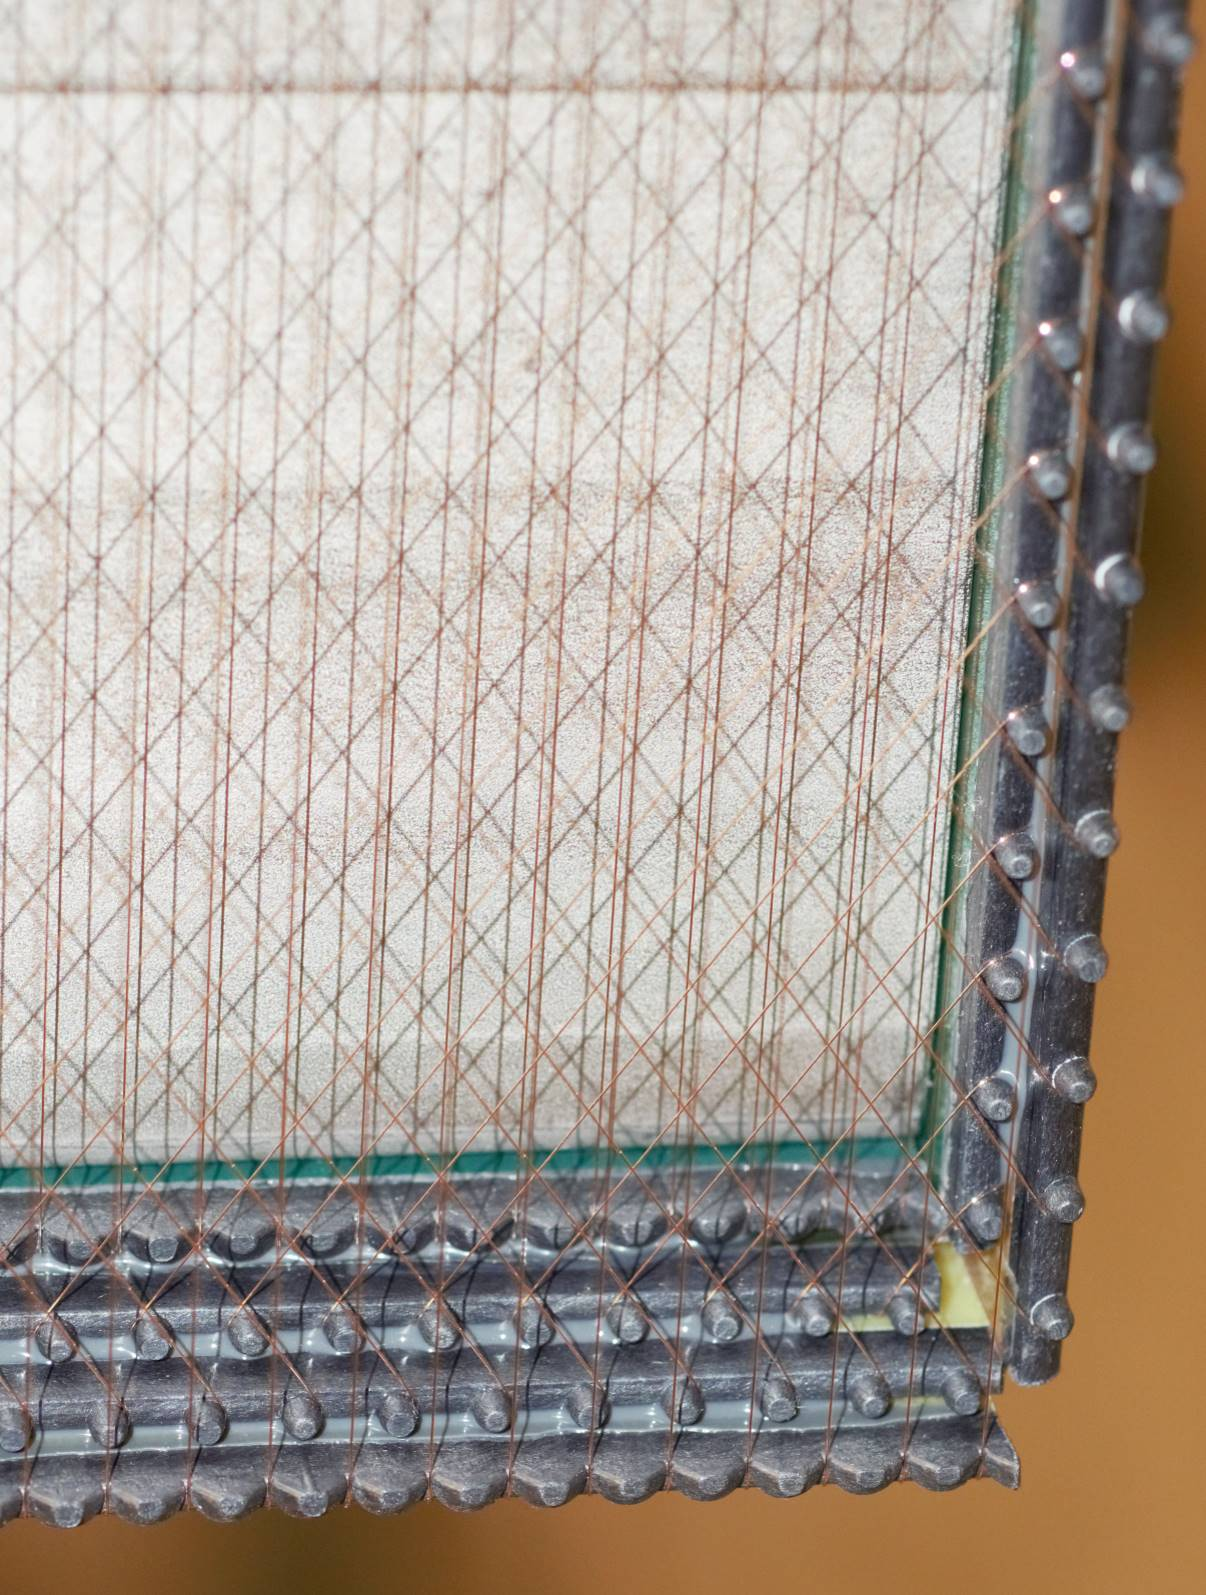
\includegraphics[height=9cm]{others/APA1-wire-photo-bo-yu.jpg}
      
      $+z_w \longleftarrow 0 \longleftarrow -z_w$
    \end{center}
  \end{minipage}

  \caption{Illustration of the three wire coordinate systems relative
    to their parent chamber coordinate system, limited to the
    transverse plane and a photo of the bottom right corner of APA1
    (Bo Yu).  For each plane \textcolor{red}{U in red},
    \textcolor{blue}{V in blue} and \textbf{W in black}, the thin
    arrows are along the wire ($y_w$) direction, the thick arrows are
    along the pitch ($z_w$) direction. The axes of the plot represent
    the $y_c$ and $z_c$ axes.  Into the page are the common $x_c$ and
    the three $x_w$ for each plane.  The photo shows grid, U, V and W
    wire planes.  Note that the illustration and the photo are viewed
    from different sides.  In the photo the $z_w$ axis points to the
    left.  The U/V wires in each representation are equivalent.}
  \label{fig:coords}
\end{figure}

\section{Connections}

The type of connections defined in the schema graph shown in
Fig.~\ref{fig:schema} require local numbering conventions so as the
children may take some order inside their parent.  This ordering must
be mapped to the physical design in order to be meaningful.  The
numbers in these conventions represent \textbf{zero-based} sequence
indices.

\subsection{Detector-APA}

The single-phase protoDUNE detector has six APAs.  The local numbering
convention for APAs in protoDUNE follow that used by the installation
group with the exception of being zero-based indices instead of
one-based counts.


\begin{table}[htp]
  
  \centering
  \begin{tabular}[h]{|c|c|c|}
    \hline
    \hline
    \hline
    5 & 4 & 3\\
    \hline
      &&\\
      &&\\
    \hline
    \hline
    \hline
      &&\\
      &&\\
    \hline
    2 & 1 & 0\\
    \hline
    \hline
    \hline
  \end{tabular}

  beam $\longrightarrow$

  \caption{Detector-APA connection indices as viewed looking down on
    the detector and following the order of the installation group
    numbering (but zero-based instead of one-based).}
  \label{tab:tpc}

\end{table}


\subsection{APA-Face-Board}

Each APA has two faces.  The first is toward a central drift volume
and identified with index zero.  The other is toward the nearby
cryostat wall and identified with index 1.  This is illustrated in
Table.~\ref{tab:anodeface}.

\begin{table}[htp]
  \label{tab:anodeface}
  \centering
  \begin{tabular}[h]{|c|c|c|}
    \hline
    \hline
    \multicolumn{3}{|c|}{croyostat}\\
    \hline
    face-1 & face-1 & face-1 \\
    \hline
    \hline
    face-0 & face-0 & face0 \\
    \hline
    \multicolumn{3}{|c|}{}\\
    \multicolumn{3}{|c|}{central drift volume}\\
    \multicolumn{3}{|c|}{}\\
    \hline
    \hline
    \hline
    \multicolumn{3}{|c|}{}\\
    \multicolumn{3}{|c|}{central drift volume}\\
    \multicolumn{3}{|c|}{}\\
    \hline
    face-0 & face-0 & face0 \\
    \hline
    \hline
    face-1 & face-1 & face-1 \\
    \hline
    \multicolumn{3}{|c|}{cryostat}\\
    \hline
    \hline
    \multicolumn{3}{c}{beam $\longrightarrow$} \\    

  \end{tabular}
  \caption{Anode-face connection indices.  Regardless of the APA, face-0 is toward the central drift volume.}
\end{table}

Within each face are ten cold electronics boxes holding associated
with a colde front-end electronics board or equivalently a wire board.
Theses boxes are numbered 0-9 in left-to-right order when looking at a
given face.  Although numbered differently, these are shown in
Fig.~\ref{fig:wibflange}.  The blue and red dots labeled b1-b10
represent boxes 0-9 on face-0 and those labeled b11-b20 are boxes 0-9
on face-1.

\subsection{APA-WIB-Board}

An APA has a single warm electronics crate with five slots, each
holding one WIB.  Each WIB has four connectors to one board.
Table~\ref{tab:femb-wib-1} shows the WIB-board connectivity map.
Figure~\ref{fig:wibflange} shows their physical layout on the warm
interface flange.  

\begin{table}[htp]
  \label{tab:femb-wib-1}
  \centering
  \begin{tabular}[h]{|c|c|c|c|c|c|c|c|c|c|}
    \hline
    \multicolumn{10}{|c|}{Cryostat wall} \\
    \hline
    WIB 5 & WIB 4 & WIB 3 & WIB 2 & WIB 1 & WIB 5 & WIB 4 & WIB 3 & WIB 2 & WIB 1 \\
    \multicolumn{5}{|c|}{WIB connector 4} & \multicolumn{5}{c|}{WIB connector 3} \\
    \hline
    \multicolumn{10}{|c|}{APA Frame} \\
    \hline
    \multicolumn{5}{|c|}{WIB connector 1} & \multicolumn{5}{c|}{WIB connector 2} \\
    WIB 1 & WIB 2 & WIB 3 & WIB 4 & WIB 5 & WIB 1 & WIB 2 & WIB 3 & WIB 4 & WIB 5\\
    \hline
    \multicolumn{10}{|c|}{TPC} \\
    \hline
  \end{tabular}
  \caption{FEMB-WIB connectivity proposal \#1.  The table shows mapping from the $2\times10$ physical FEMB location on the top of the APA to WIB addresses following a $1\times5\times4$ layout.}
\end{table}

This layout allows for a simple mapping to be iterated over in code
and in particular allows simple separation and enumeration of
collection channels from each face.  A second layout based on
$2 \times 2 \times 5$ blocks of boards was considered but was
considered slightly less preferable due to the somewhat higher
complexity.



\begin{figure}[h]
  \centering
  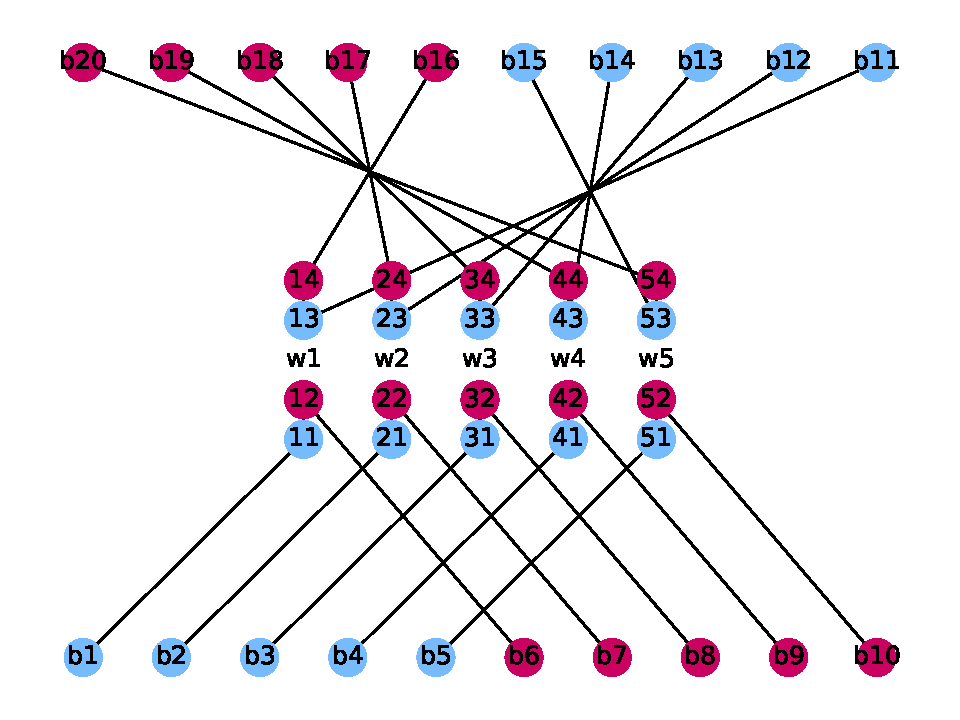
\includegraphics[height=7cm]{test_plot_wib.pdf}%
  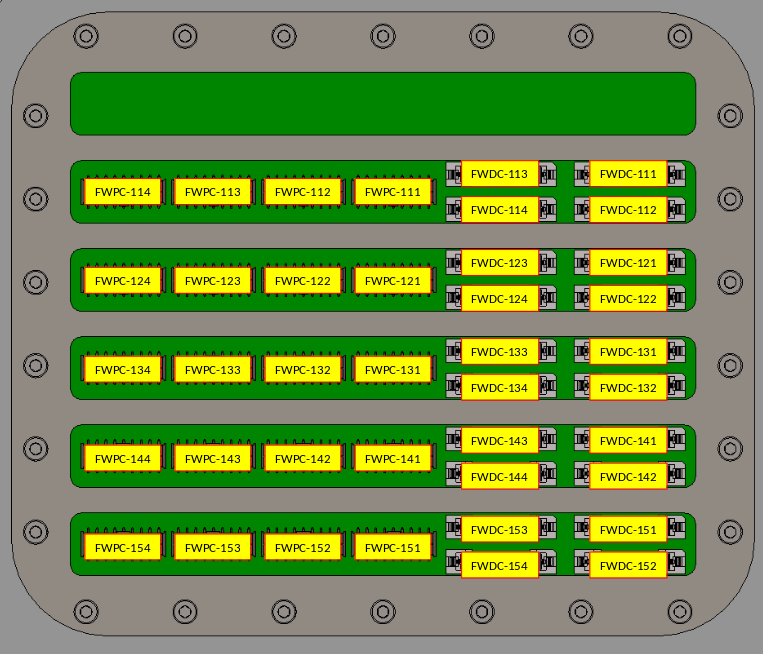
\includegraphics[height=7cm]{others/manhong-ce-mapping-wib.png}

  \caption{On the left, logical connections between boards in cold
    electronics boxes lined up on either face of an APA and the warm
    interface board connectors. Note these numbers are
    \textbf{one-based counts and not zero-based indices} such as used
    in the connectivity graph.  On the right, a drawing from Manhong
    showing front-end power and data connectors through the warm
    interface flange.  The filled circles on the left marked b1-b10
    represent CE boxes on APA (front) face-0 and b11-b20 on (back)
    face-1.  The points marked w1-w5 represent the five WIBs with each
    of their connectors shown above and below and numbered to match
    the data connectors on the warm interface flange.}
  \label{fig:wibflange}
\end{figure}

\subsection{Board-Chip-Channel-Conductor}

Each board has eight chips and each chip has 16 channels each of which
connects to one conductor.  The conductor is also identified with a
row and a spot on a wire board.  Each row is identified with one plane
of a face and the spots in a row are identified with a sequence of
wires.  The complex shuffle between the pair (chip, channel) and the
pair (row, spot) is summarized in Table~\ref{tab:wirechmap}.
This connection is visualized in Figure~\ref{fig:boardchip}.

\begin{table}[htp]
  \label{tab:wirechmap}
  \centering

  % generated by chmap.py using files:
% others/shanshan/ProtoDUNE_APA_Wire_Mapping_091917_v3-J1.csv
% others/shanshan/ProtoDUNE_APA_Wire_Mapping_091917_v3-J2.csv
\begin{tabular}{r|rrrrrrrr}
\hline
ASIC:&1&2&3&4&5&6&7&8\\
\hline
ch00 & \textcolor{red}{u19} & \textcolor{red}{u09} & \textcolor{black}{w14} & \textcolor{black}{w02} & \textcolor{red}{u29} & \textcolor{red}{u39} & \textcolor{black}{w26} & \textcolor{black}{w38}\\
ch01 & \textcolor{red}{u17} & \textcolor{red}{u07} & \textcolor{black}{w16} & \textcolor{black}{w04} & \textcolor{red}{u27} & \textcolor{red}{u37} & \textcolor{black}{w28} & \textcolor{black}{w40}\\
ch02 & \textcolor{red}{u15} & \textcolor{red}{u05} & \textcolor{black}{w18} & \textcolor{black}{w06} & \textcolor{red}{u25} & \textcolor{red}{u35} & \textcolor{black}{w30} & \textcolor{black}{w42}\\
ch03 & \textcolor{red}{u13} & \textcolor{red}{u03} & \textcolor{black}{w20} & \textcolor{black}{w08} & \textcolor{red}{u23} & \textcolor{red}{u33} & \textcolor{black}{w32} & \textcolor{black}{w44}\\
ch04 & \textcolor{red}{u11} & \textcolor{red}{u01} & \textcolor{black}{w22} & \textcolor{black}{w10} & \textcolor{red}{u21} & \textcolor{red}{u31} & \textcolor{black}{w34} & \textcolor{black}{w46}\\
ch05 & \textcolor{blue}{v19} & \textcolor{blue}{v09} & \textcolor{black}{w24} & \textcolor{black}{w12} & \textcolor{blue}{v29} & \textcolor{blue}{v39} & \textcolor{black}{w36} & \textcolor{black}{w48}\\
ch06 & \textcolor{blue}{v17} & \textcolor{blue}{v07} & \textcolor{blue}{v12} & \textcolor{blue}{v02} & \textcolor{blue}{v27} & \textcolor{blue}{v37} & \textcolor{blue}{v22} & \textcolor{blue}{v32}\\
ch07 & \textcolor{blue}{v15} & \textcolor{blue}{v05} & \textcolor{blue}{v14} & \textcolor{blue}{v04} & \textcolor{blue}{v25} & \textcolor{blue}{v35} & \textcolor{blue}{v24} & \textcolor{blue}{v34}\\
ch08 & \textcolor{blue}{v13} & \textcolor{blue}{v03} & \textcolor{blue}{v16} & \textcolor{blue}{v06} & \textcolor{blue}{v23} & \textcolor{blue}{v33} & \textcolor{blue}{v26} & \textcolor{blue}{v36}\\
ch09 & \textcolor{blue}{v11} & \textcolor{blue}{v01} & \textcolor{blue}{v18} & \textcolor{blue}{v08} & \textcolor{blue}{v21} & \textcolor{blue}{v31} & \textcolor{blue}{v28} & \textcolor{blue}{v38}\\
ch10 & \textcolor{black}{w23} & \textcolor{black}{w11} & \textcolor{blue}{v20} & \textcolor{blue}{v10} & \textcolor{black}{w35} & \textcolor{black}{w47} & \textcolor{blue}{v30} & \textcolor{blue}{v40}\\
ch11 & \textcolor{black}{w21} & \textcolor{black}{w09} & \textcolor{red}{u12} & \textcolor{red}{u02} & \textcolor{black}{w33} & \textcolor{black}{w45} & \textcolor{red}{u22} & \textcolor{red}{u32}\\
ch12 & \textcolor{black}{w19} & \textcolor{black}{w07} & \textcolor{red}{u14} & \textcolor{red}{u04} & \textcolor{black}{w31} & \textcolor{black}{w43} & \textcolor{red}{u24} & \textcolor{red}{u34}\\
ch13 & \textcolor{black}{w17} & \textcolor{black}{w05} & \textcolor{red}{u16} & \textcolor{red}{u06} & \textcolor{black}{w29} & \textcolor{black}{w41} & \textcolor{red}{u26} & \textcolor{red}{u36}\\
ch14 & \textcolor{black}{w15} & \textcolor{black}{w03} & \textcolor{red}{u18} & \textcolor{red}{u08} & \textcolor{black}{w27} & \textcolor{black}{w39} & \textcolor{red}{u28} & \textcolor{red}{u38}\\
ch15 & \textcolor{black}{w13} & \textcolor{black}{w01} & \textcolor{red}{u20} & \textcolor{red}{u10} & \textcolor{black}{w25} & \textcolor{black}{w37} & \textcolor{red}{u30} & \textcolor{red}{u40}\\
\hline
\end{tabular}


  \caption{The per-board connections between a chip (columns) and its
    channel (rows, one-based count) and the local numbering the row
    and spot for a conductor connection.  The row is identified by a
    plane letter (``u'', ``v'' or ``w'') and the spot is a numbered
    count starting from one (not zero).  Counts are
    \textcolor{red}{1-40 for U plane and marked in red},
    \textcolor{blue}{1-40 for V plane and marked in blue} and
    \textbf{1-48 for W plane and marked in black}.  This pattern is
    applied for each board on each face of an APA.}
\end{table}


\begin{figure}[h]
  \centering
  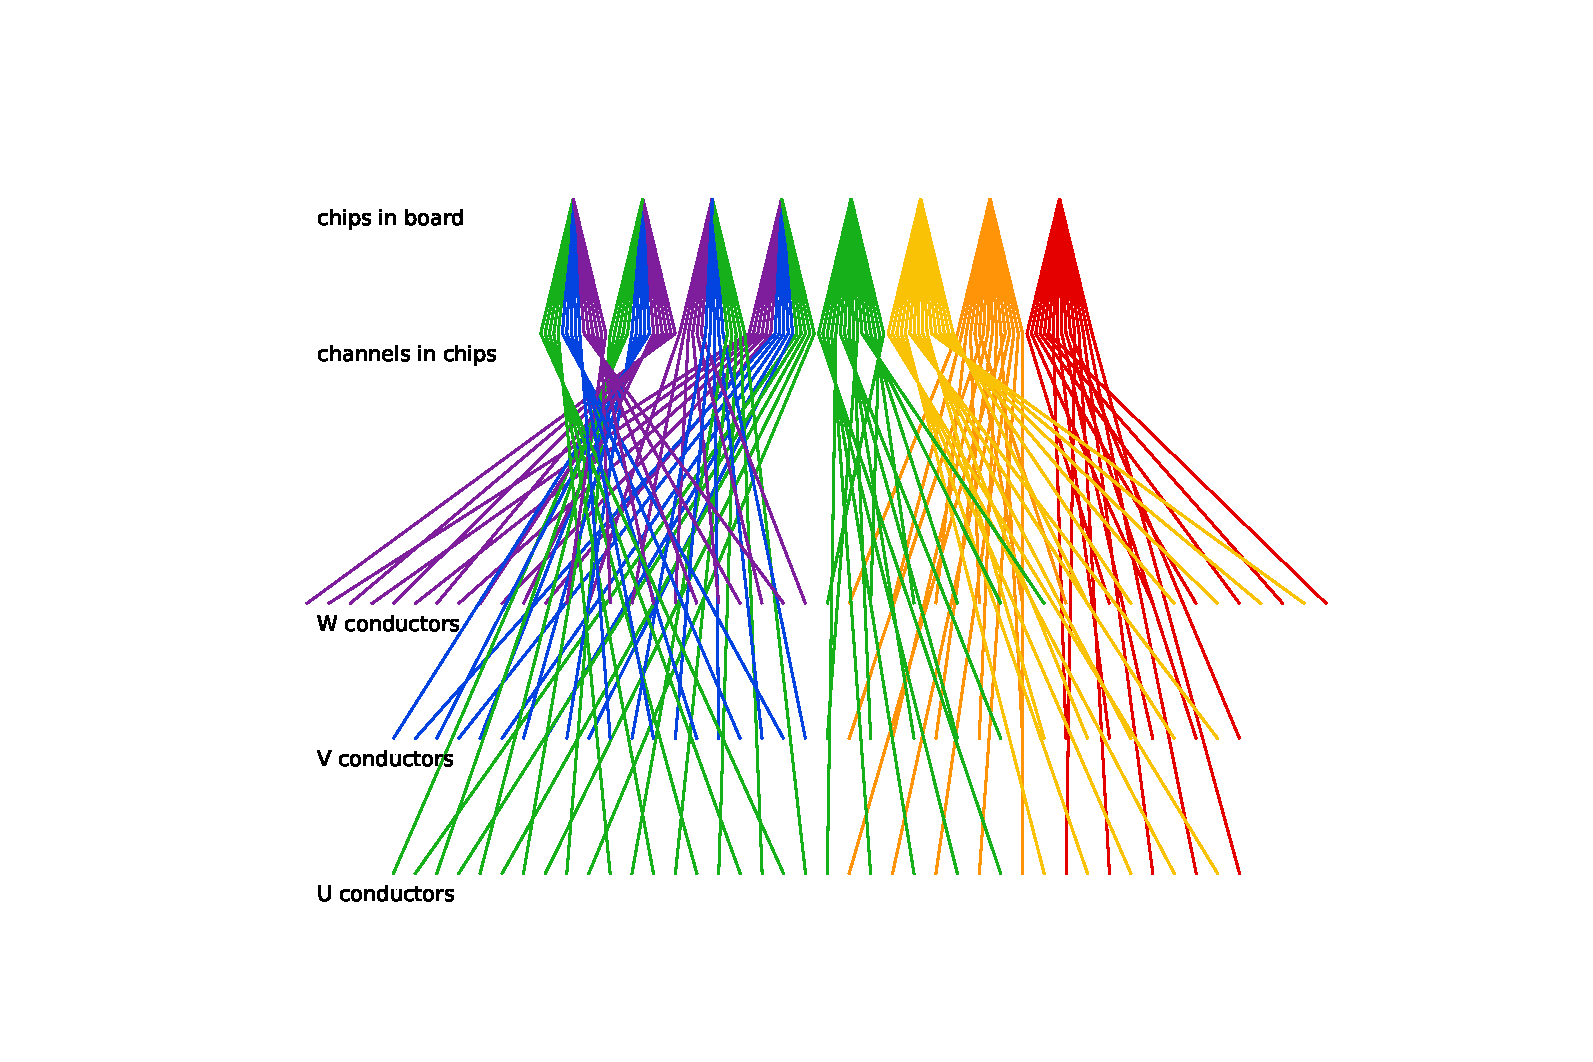
\includegraphics[width=\textwidth]{test_plot_board_chip.pdf}
  \caption{Visualization of the connectivity between the channels of the eight chips on one board and the conductors attaching at a given spot in a row on the associated wireboard.  The channels of the first four chips are colored according to the wire board row (plane) they service.  The channels from the last four chips are colored by their chip number.}
  \label{fig:boardchip}
\end{figure}


\subsection{Conductor-Wire}

Figure~\ref{fig:wires} visualizes a subset of wire segments separated
by planes in an APA face.  They are drawn consistent with
Fig.~\ref{fig:coords} and in particular with the same caution that one
is viewing the wires looking in the direction counter to the nominal
electron drift.  In all cases the index of a wire in its plane is
counted starting for the wire with its center at the most negative Z
location which also corresponds to the wire with the most negative
pitch location.  For the U plane, wire-0 is at the top of the APA, for
the V plane it is at the bottom.  Note, this convention has the
wire-in-plane index run generally counter the direction that a face's
boards or a board's conductor spots are numbered.  


\begin{figure}[htp]
  \centering
  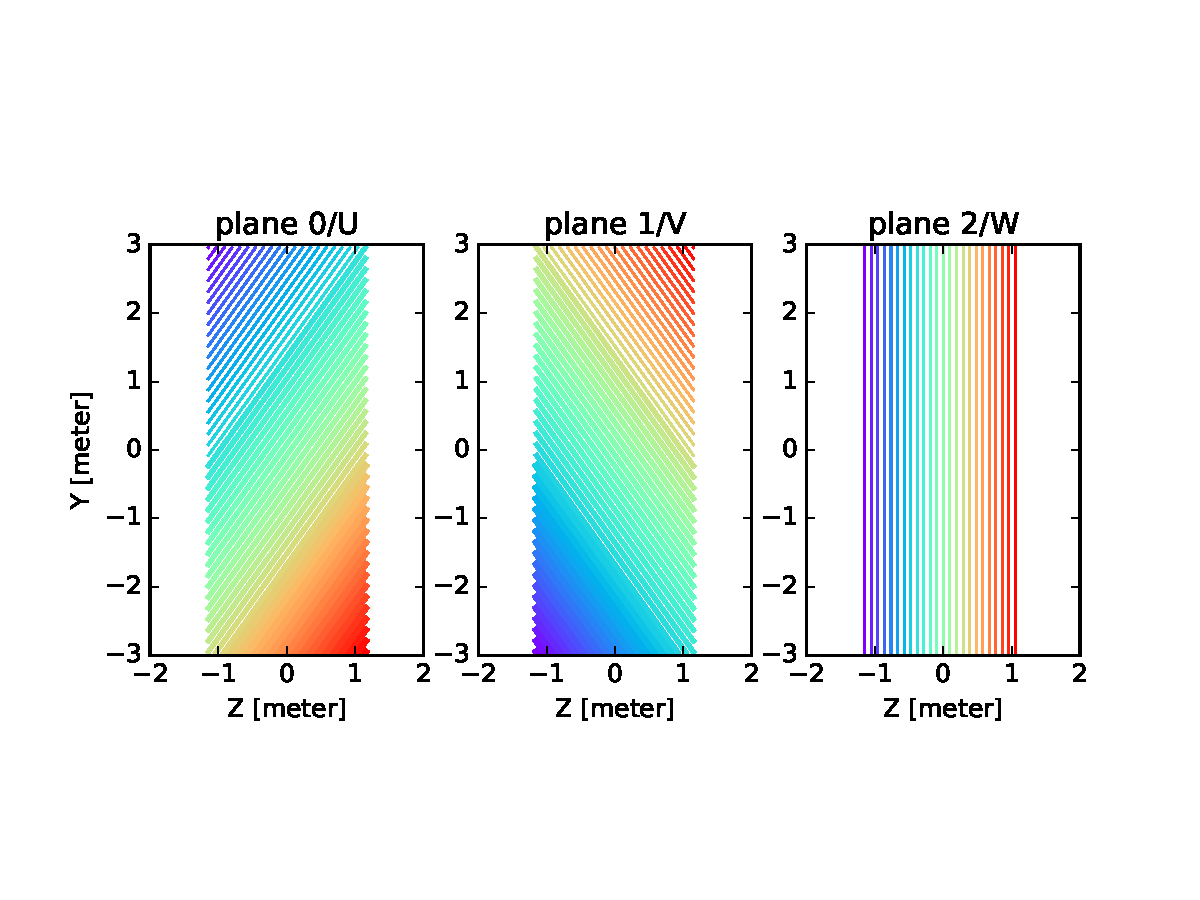
\includegraphics[width=\textwidth,clip,trim=0 3cm 0 3cm]{wires-20.pdf}
  \caption{The wire (segments) for each wire plane on one face of one APA for protoDUNE.  Increasing line width indicates increasing \textbf{segment number} $\in$ (0, 1 or 2).  The color indicates increasing \textbf{wire index} from blue to red.  Only one of every twenty wires are shown. The Y coordinate points opposite of gravity.  The unlabeled X coordinate runs into the page and is counter to the drift direction.  Z follows from the right-hand-rule.}
  \label{fig:wires}
\end{figure}


\subsection{Board-Chip-Conductor-Wire}

Each board services 128 conductors.  These conductors may wrap around
zero, once or twice depending on which plane they are in and where the
conductors enter the plane.  Figure~\ref{fig:board} visualizes the
location of the wires from each of the ten boards on one face.

\begin{figure}[h]
  \centering
  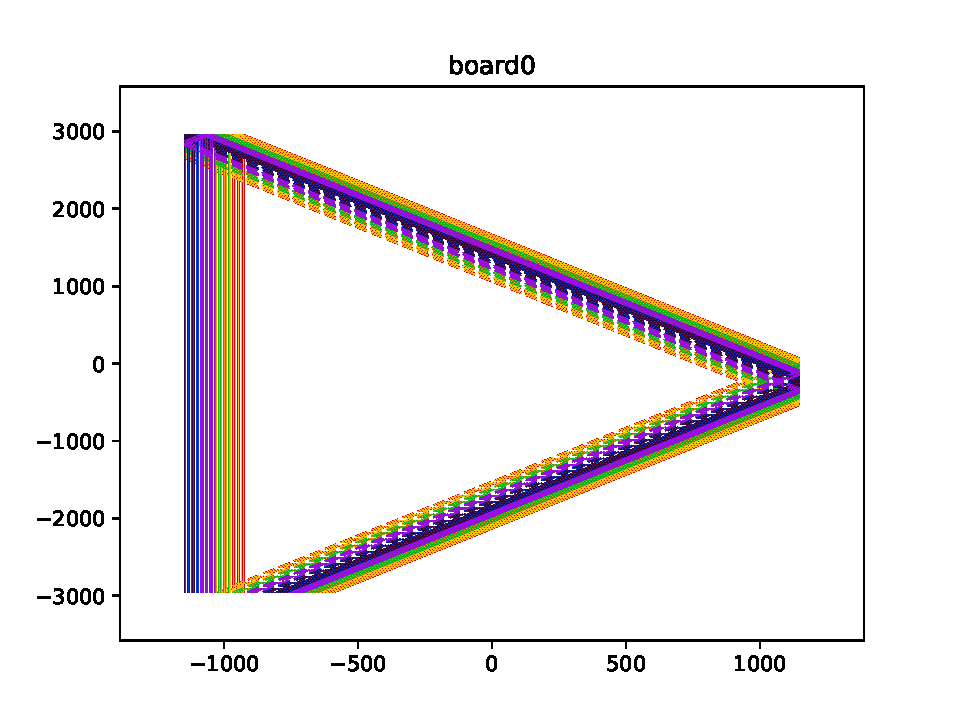
\includegraphics[width=0.5\textwidth,page=1]{test_plot_board.pdf}%
  \includegraphics[width=0.5\textwidth,page=2]{test_plot_board.pdf}

  \includegraphics[width=0.5\textwidth,page=3]{test_plot_board.pdf}%
  \includegraphics[width=0.5\textwidth,page=4]{test_plot_board.pdf}

  \includegraphics[width=\textwidth,page=3,clip,trim=3cm 8cm 8cm 2cm]{test_plot_board.pdf}

  \caption{The location of wires, in chamber coordinates ($z_c,y_c$)
    for the first four boards on a face.  Wires are colored by the
    chip in which their conductor is connected.  Wires that are
    wrapped around to the other face are dashed.  Note: depending on
    the technology used to view this image, many fine details may be
    obscured.  The fifth plot shows a zoom into the top left corner of
    the third board (``board2'').}
  \label{fig:board}
\end{figure}


\section{Global Numbering}

The numbers described above are local to each type of connection.
They require adopting a minimal convention in order to associate them
to real-world connections.  It is often useful to flatten the graph to
an ordered sequence of identifiers which are unique in some context.

For example, LArSoft requires an exhaustive list of every wire segment
across the entire detector and it assumes ``channel'' numbers which
are conceptually more similar to the conductor attachment spots on
wire boards.

Such special case conventions can be accommodated by writing a
function that traverses the full connectivity graph and applies some
transformation to its minimal numbering convention in order to produce
identifiers in the desired scheme.

\section{Software}

The software used to generate the full connection graph, up to one APA
is available in the
\href{https://github.com/wirecell/wire-cell-python}{wire-cell-python}
package.  This is a pure Python package developed in support of the
C++ Wire-Cell Toolkit (WCT).  It can be installed and run like any
Python package and in particular, independent from the WCT C++
packages.

To generate the connection graph using default parameters code like
the following is used.

\begin{verbatim}
  from wirecell.util.wires import apa
  desc = apa.Description();
  G,P = apa.graph(desc)
\end{verbatim}

The returned value \texttt{G} is a
\href{https://networkx.github.io/}{NetworkX} graph and as such can be
used for any number of graph-theoretic operations including persisting
it to many supported formats.

The returned value \texttt{P} is a simple named tuple allowing easy
access to nodes of the different types in the order in which they were
created.

The \texttt{apa.Description} class constructor takes an optional set
of parameters defaulting to \texttt{apa.default\_params}.  These
parameters govern such things as:

\begin{itemize}
\item Wire angles, pitch, starting location
\item Plane width, height, location
\item Multiplicity of boards, WIBs, their connectors, chips and channels
\item Chip/channel mapping to conductor row and spot.
\end{itemize}

\end{document}

%%% Local Variables:
%%% mode: latex
%%% TeX-master: t
%%% End:
